\announcesection{Results}

\frame{
    \frametitle{Basic Poisson Statistics with Event Yields}
    {\scriptsize
    With signal and background, Poisson expectation is $\mu S + B$
    \vspace{2mm}

    \begin{table}[tbh]
       \begin{center}
           \begin{tabular}{|l|l|l|}
           \hline
               Type  &	Event Yield & p-value \\
                     &$200 < m_{HH} < 1400$ & \\
               \hline
               Background Estimate        & 493.6 & \\
               Signal Hypothesis (SM)     & 0.36  & \\
               Signal Hypothesis (\kvv=3) & 52.7  & \\
               Observed Data              &    & \\
           \hline
           \end{tabular}
       \end{center}
    \end{table}
    }
    \vspace{0.8\textheight}
}

\displaytwo{Basic Poisson Statistics with Event Yields}{
    {\scriptsize
    With signal and background, Poisson expectation is $\mu S + B$
    \vspace{2mm}

    \begin{table}[tbh]
       \begin{center}
           \begin{tabular}{|l|l|l|}
           \hline
               Type  &	Event Yield & p-value \\
                     &$200 < m_{HH} < 1400$ & \\
               \hline
               Background Estimate        & 493.6 & 0.54 \\
               Signal Hypothesis (SM)     & 0.36  & 1.15 \\
               Signal Hypothesis (\kvv=3) & 52.7  & 0.03 \\
               Observed Data              & 495   & N/A  \\
           \hline
           \end{tabular}
       \end{center}
    \end{table}
    \vspace{2mm}

    P-value of signal calculated as:
    $P_S = \frac{P_{S+B}}{1 - P_B}$
    }
}
{results/total_yield_poisson_1p00_1p00_1p00}
{results/total_yield_poisson_3p00_1p00_1p00}

\displayonecenter{$\mu S + B$: $\mu$-Scanning}{{\footnotesize
    \framesubtitle{Total Event Yields and Statistical Errors \textbf{Only}}
    Can asign a value of how (un)-reasonable a particular signal is,
        by determining how much that signal would need to be scaled (by $\mu$)
        in order to be excluded to 95\% confidence
}}{results/mu_pvalue_1p00_1p00_1p00}

\displayonecenter{$\mu S + B$: $\mu$-Scanning Elswhere}{
    \framesubtitle{Total Event Yields and Statistical Errors \textbf{Only}}
    {\footnotesize
    A 95\% confidence at a $\mu<1$ indicates the observed data cannot accomodate the hypothesized excess signal yield
    }
}{results/mu_pvalue_3p00_1p00_1p00}

\displayonecenter{One-Dimensional Limits for \kvv}{
    \framesubtitle{Total Event Yields and Statistical Errors \textbf{Only}}
    {\footnotesize
    Plotting the 95\% confidence $\mu$ as a function of \kvv shows the precise value
    at which \kvv can be excluded.
    }
}{results/mu_limits_fast_k2v}

\displayonecenter{2D-Limits}{
    \framesubtitle{Total Event Yields and Statistical Errors \textbf{Only}}
    {\footnotesize
    The exclusion points specifically can viewed as a function of both \kvv and \kl
        (with \kv fixed to 1)
    }
}{results/limit_slice_kv_1p0}

\displaythree{More 2D-Limits}{
    \vspace{-4mm}
    {\usebeamercolor[fg]{subtitle} \footnotesize Total Event Yields and Statistical Errors \textbf{Only}}
    \vspace{3mm}

    The full 3D limits can be viewed in slices with different $\kappa$'s fixed
}{results/limit_slice_kv_1p0}
{results/limit_slice_kl_1}
{results/limit_slice_k2v_1p0}

\frame{
    \frametitle{Full 3D Coupling Limits}
    \framesubtitle{Total Event Yields and Statistical Errors \textbf{Only}}
    \begin{figure}
        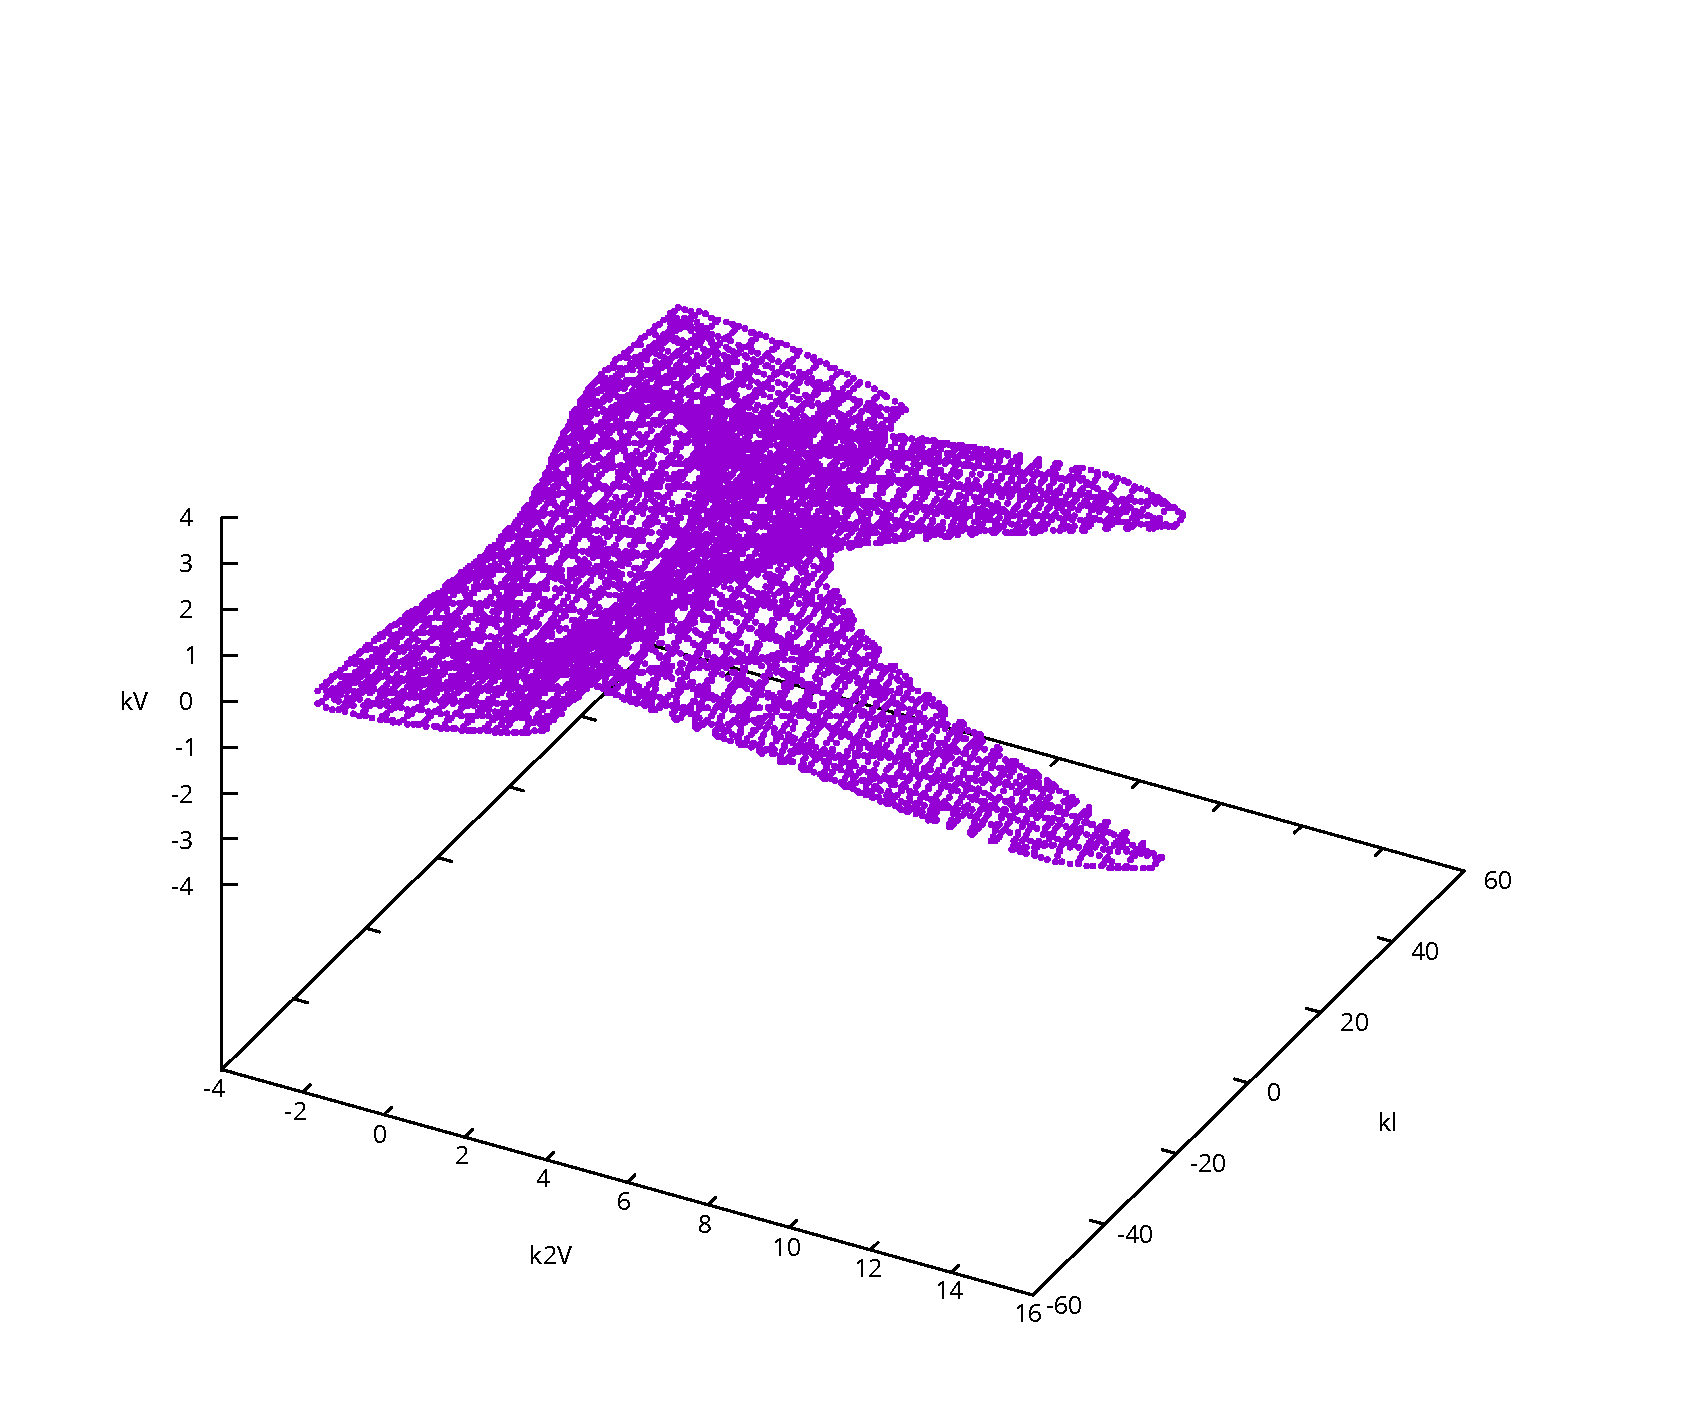
\includegraphics[width=\linewidth,height=0.9\textheight,keepaspectratio]{results/full_3D_point_cloud}
    \end{figure}
}

\displayonelarge{\mhh Significance}{
    Binning events by \mhh permits greater ``significance'':
    \vspace{3mm}

    $Z_s=\frac{S}{\sqrt{S+B}}$
}
{results/data_dump_m_hh_3p00_1p00_1p00}

\displayonelarge{$\deta_{hh}$ Significance}{
    A similar effect can be achieved with $\deta_{hh}$
}
{results/data_dump_dEta_hh_3p00_1p00_1p00}



\frame{
    \frametitle{Log Likelihood Profile Fit}

    Two categories ($j=[1,2]$), for $\deta_{hh} < 1.5$ and $\deta_{hh} > 1.5$
    \vspace{3mm}

    Four nuissance parameters ($a=[1,4] $) for each of the four background shape uncertainties
    \vspace{3mm}

    {\footnotesize
        \begin{equation} \begin{split}
            P_{\textrm{poiss}}(n_i | \nu_i) =  \frac{ (\mu S_i + \Theta B_i)^{n_i} e^{\mu S_i + \Theta B_i} }{n_i!}
            \nonumber
        \end{split} \end{equation}
    }

    {\footnotesize
        \begin{equation} \begin{split}
                 P_{\textrm{gauss}}(n_i | \nu_i, \sigma_i^a) = \frac{1}{\sigma_i^a \sqrt{2\pi}} e^{
                    -\frac{1}{2}\left(\frac{n_i- (\mu S_i + \Theta B_i)}{\sigma_i^a}\right)^2
                }
            \nonumber
        \end{split} \end{equation}
    }

    \begin{equation}
        L(n,\mu,\Theta) = \prod \limits_{j=1}^{2}
             \prod \limits_{i=1}^{N} P_{\textrm{poiss}}(n_{ij} | \nu_{ij}) 
             \prod \limits_{a=1}^{4} P_{\textrm{gauss}}(n_{ij} | \nu_{ij}, \sigma_{i}^a) 
        \nonumber
    \end{equation}
}


\displayonecenter{\kvv $\mu$-Scan and Expected Limits}{
    Use null hypothesis to predict what limits should look like,
    observe for large unexpected deviations that could indicate
    errors or exotic physics.
}{results/k2v_scan_thesis_final0_1D_k2v_samps_vbf_pd_vbf_inc161718_kl_1.0_mu}


\displayonecenter{\kvv Cross-Section Limits}{
    Multiply $\mu$ by theoretical cross-section to place
        upper bound on the \vbfproc cross-section
        and assign limits to \kvv.
}{results/k2v_scan_thesis_final0_1D_k2v_samps_vbf_pd_vbf_inc161718_kl_1.0_xs}


\displayonecenter{\kl Cross-Section Limits}{}
{results/kl_scan_thesis_final0_1D_kl_samps_vbf_pd_vbf_inc161718_k2v_1.0_xs}


% Emphasize "exclusion"
\displaytwo{$\kvv/\kl$ and $\kvv/\kv$ 2D Limits}{
    This analysis can exclude everything grey
        (\textit{outside} the black boudaries)
        to 95\% confidence.
}{results/2D_scan_thesis_omega0_kvv_kl_samps_vbf_pd_vbf_inc161718_k1v1p00_exclusion}
{results/2D_scan_thesis_omega0_kvv_kv_samps_vbf_pd_vbf_inc161718_kl1p00_exclusion}
